\chapter{ \textit{Big Data}, données biomédicales et \textit{machine-learning}}

Hiding within those mounds of data is knowledge that could change the life of a patient, or change the world
- Atul Butte, 2012

L'informatisation du monde a permis la production et l'accumulation de données de façon exponentielle. En particulier dans le domaine de la santé, les avancées technologiques comme les technologies de séquençage, d'imagerie ou les dossiers médicaux électroniques ont permis au cours du temps la capture de données précieuses pouvant améliorer le parcours et la prise en charge des patients.

Dans le même temps, les technologies d'analyse de données massives (\textit{Big-Data}) se sont développée notamment grâce au \gls{ml}, une branche de l'\gls{ia} permettant à des algorithmes informatiques d'apprendre à partir des données. Cette massification des données biomédicales et le développement des technologies d'analyse de données permet d'entrevoir un monde où les soins de santé pourraient être personalisés, préventifs et prédictifs .

Dans ce premier chapitre d'introduction nous présenterons d'abord ce que sont les big-data, la variété des données-biomédicales et comment ces données sont utile pour une meilleure prise en charge des patients.. Puis dans une seconde partie, nous présenterons les concepts principaux du \gls{ml} pour le traitement de ces données.

\section{Les données biomédicale: des \textit{Big Data} au service des patients}

\subsection{Définiton du \textit{Big-Data}}

Le terme "Big Data" est utilisé pour faire référence à l'immense quantité de données complexes et hétérogènes produites par cette informatisation du monde et le développement des technologies haut débits (\cite{de_mauro_formal_2016}). La définition des big-data a été enrichie au fur et à mesure des années d'abord par 3 mots clés puis 5 et même jusqu'à 7 (\cite{garcia_what_2022}). La définition la plus commune aujourd'hui des Big-Data se compose des 5 "V": le volume, la variété, la vélocité, la véracité et la valeur (\cite{ishwarappa_brief_2015}). Ainsi pour être considérée comme Big-Data, les données doivent: (i) être volumineuse, du gigabytes à l'exabytes, (ii) être variée c'est à dire multimodales (iii) avoir une vélocité de création et de traitement importante, (iv) être vérace, c'est à dire valide et (v) avoir une forte valeur ajoutée, c'est-à-dire qu'elle doivent être utiles. (\cite{garcia_what_2022}).

Ainsi les données biomédicales sont en adéquation à cette définition (\cite{zheng_application_2021}). Grâce aux améliorations en techniques d'acquisitions (séquençage, imagerie) elles sont volumineuses et possèdent une forte vélocité. Ces données sont variées, contenant des informations sur le plan génétique, phénotypique et histologique. De plus elle ont un véracité assurée couplée à une forte valeur ajoutée. En effet ce sont de manière général des données générée par des experts (médecin ou biologiste) et liées à des patients (et donc fortement valorisées). Il est alors juste de parler de qualifier les données biomédicales de Big-Data (\cite{sonawane_network_2019}. Ainsi dans la prochaine section nous allons voir en détails les différents modalités de données biomédicales de patients, leur acquisitions et les challenges que présentent leur analyse.

\subsection{Variété des données biomédicales}
Les données biomédicales sont par nature multimodales (\cite{acosta_multimodal_2022}). Le diagnostic d'un patient peut se réaliser par l'intégration de différents niveau d'informations. Tout d'abord il y a les données phénotypiques, listant les symptômes et autre caractéristiques du patient après un examen médical. Ces données sont souvent sous la forme de texte libre, rédigé par le praticien de santé. Ensuite les données d'imagerie, issues le plus souvent d'examens complémentaire pour mieux caractériser l'atteinte du patient (échographie, IRM, histopathologie). Et enfin il y a les données génétiques et omiques, qui sont nécessaires dans le cadre de maladie génétiques pour cibler les dysfonctionnement d'origine génétiques (données de types séquences). Ce trio texte libre, imagerie et séquences implique des techniques d'acquisition, de traitement et des difficultés propres.

\subsubsection{Données textuelles et dossiers de santé électroniques}
Les données en texte libre sont très commune dans le cadre des données de santé. Un rendez-vous, un examen complémentaire ou un échange entre confrères, peuvent donner lieu à la rédaction de comptes rendus médicaux en texte libre contenant des informations expertisées et hautement valorisée concernant le diagnostic du patient. De plus, la rédaction de comptes-rendus ne nécessite pas de technologie d'acquisition particulière, ce qui a permis l'accumulation au cours du temps d'archive de comptes-rendus médicaux massive qui restent à explorer.

Dans le cadre de cette volonté d'explorer ces données, les \gls{dse} sont des outils pour numériser ces comptes-rendus textuels afin de les centraliser et les exploiter (\cite{graber_impact_2017}). Cependant le développement d'outils pour numériser et exploiter les comptes rendus en texte libre est difficile. La compréhension du texte libre par un programme informatique est une tâches ardue. C'est pourquoi la majorité des solutions de \gls{dse} demandent une phase d'annotation manuelle (remplissage de formulaires et de champs) par l'utilisateur pour numériser les données, ce qui est pratique est rarement réalisé faute de temps.

\subsubsection{Données d'imagerie: microscopie à haute résolution}
Le développement des techniques d'imagerie a permis une diversification des techniques d'imagerie (IRM, échographie, microscopie optique et électronique, imagerie 2D et 3D...) tout en améliorant leur résolutions et précision de capture  et en réduisant les coûts associés (\cite{abdallah_history_2017, prakash_super-resolution_2022, sheppard_structured_2021}). Ainsi l'imagerie médicale est devenue un examen de routine pour le diagnostic de divers pathologies. Cette production de données d'imagerie en routine et de grande résolution ont donné lieu à une massification des données d'imagerie. Ainsi il peut-être pour un clinicien d'évaluer manuellement ces données de manière exhaustive. Le développement d'outils capable d'analyser et de quantifier les éléments d'intérêt sur les données d'imagerie est donc un enjeu majeur (\cite{tchito_tchapga_biomedical_2021}) pour à la fois accélérer l'évaluation des données d'imagerie mais aussi pour améliorer la précision des cliniciens. Par exemple, dans le cadre de la microscopie photonique, il est maintenant courant d'utiliser des scanner de lame complète, générant ainsi des images à l'échelle du gigabytes par lame. Ces images sont extrêmement coûteuses en temps s'il on veut réaliser une évaluation manuelle exhaustive et un comptage des caractéristiques pathologiques en vue d'un diagnostic.

\subsubsection{Données génétiques et omiques}
Enfin, les progrès en termes de technologies de séquençage grâces notamment aux technologie de seconde génération à lecture courtes (technologie Illumina) et aux technologie de troisième générations à lecture longue (technologie PacBio et Nanopore) ont permis l'accès à l'ensemble des informations génétiques et omiques de l'Homme. De plus la baisse des coûts de séquençage, rend possible l'utilisation de séquençage de génome complet pour le diagnostic de maladies génétique chez les patients (\cite{rabbani_next-generation_2012}). Plus récemment, les techniques dites "omiques" (figure \ref{fig:intro-omics}, \cite{momeni_survey_2020}) sont utilisée pour mieux comprendre les pathologiques tels que les technologies de tanscriptiomiques (expression ARN des gènes), épigénétiques, protéomiques (expression protéiques des gènes) et métabolomiques (étude des métabolites). Ces technologies d'obtenir une vue globales de mécanismes biologiques qui opèrent au sein d'un tissus. 
\begin{figure}[!htbp]
 \centering
 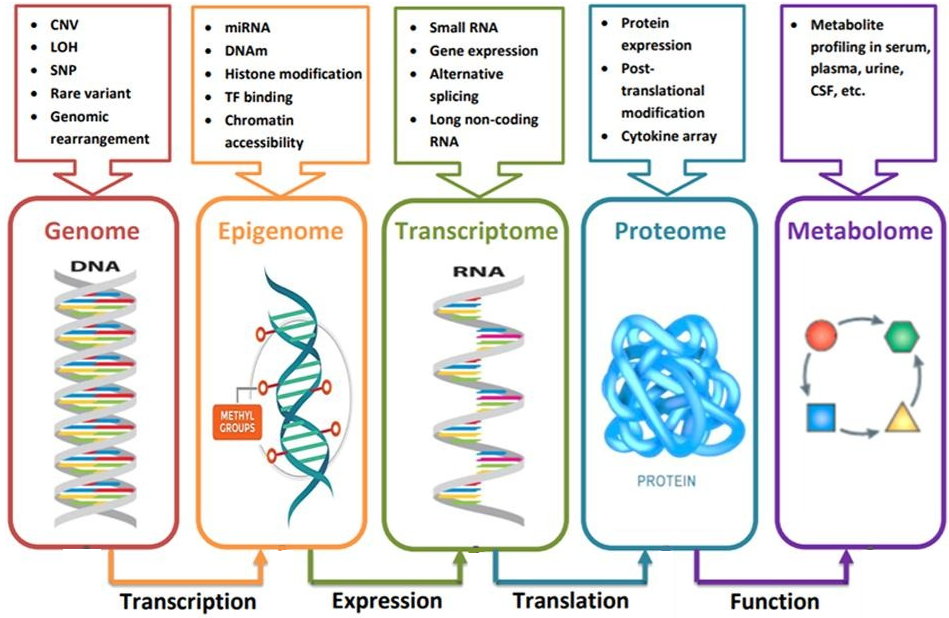
\includegraphics[width=1\textwidth]{figures/intro_omics.png}
 \caption[Méthodes de séquençages "omiques"]{Schéma des différentes méthodes de séquençages "omiques" donnant accès à une vue globales des mécanismes biologiques dans les tissues biologiques. (Modifié de \cite{momeni_survey_2020})}
 \label{fig:intro-omics}
\end{figure}
Les données de séquençages sont massives, le génome humaine mesurant environ 3.1 miliards de paires de bases (bp), le séquençage d'un génome unique avec une profondeur de 50X (nécessaire pour la détection de mutation génétique) représente un minimum de 150 miliards de paires de bases lues et stockées, pour un individus. Ces données de séquence massives, requiert des outils spécifique et un matériel informatique adapté à leur traitement. De plus la détection de mutations pathogène est complexe. L'identification du gène responsable d'une maladie génétique reste un challenge lors du diagnostique, même avec les données de séquençage complètes.

La collecte et l'intégration de l'ensemble de ces données biomédicales générées grace aux nouvelles tehcnologies haut-débit en imagerie, séquençage et \gls{dse} ont le potentiel d'améliorer la compréhension des maladies et la prise en charge des patients.

\subsection{Collecte et utilisation des données biomédicales au service du patient}
Le Royaume-Uni est un pays pionnier dans la collecte et la mise à disposition de façon massive de données biomédicales à travers le \gls{nhs}. Cela s'illustre par exemple par le projet 100 000 génomes, lancé en 2012 qui a pour but de séquencer 100 000 génomes de patient anglais pour améliorer la recherche et le diagnostic de maladie rares, certains cancers et maladies infectieuses (\cite{nunn_public_2019}). En avril 2022 a été publié le rapport de 112 pages intitulé: "\textit{Better, broader, safer: using health data for research and analysis}" (\cite{ben_goldacre_better_2022}), écrit par le professeur Ben Goldacre missioné par le \gls{nhs}. Ce rapport mets en évidence le challenge et la stratégie à adopter pour une collecte et un usage à grand échelle de données biomédicales de patients. Le projet OpenSAFELY (\href{https://www.opensafely.org/}{https://www.opensafely.org/}), fondé par Ben Goldacre, est un exemple concret d'utilisation de données biomédicales au service de la recherche et de la prise en charge de patients. Ce projet, créé en juin 2020 pour lutter contre la pandémie de COVID-19, mets à disposition des chercheurs des outils et des données biomédicales massives de patients. A ce jour, ce projet a permis la publication des plus de 80 publications scientifique de recherches réalisés à partir de ces données. Des initiatives similaires  mettent en évidence l'utilité des big-data biomédicales comme catalyseur de découvertes scientifiques, tel que le projet "Big Data to Knowledge" fondé par le \textit{National Institutes of Health (NIH)} (\cite{toga_big_2015}).

Outre la phase de collecte, la difficulté dans l'exploitation des données biomédicale réside dans la disponibilité techniques d'analyse adaptées (\cite{wang_big_2019, ismail_requirements_2020}). Les données biomédicales étant volumineuses, complexes et multimodales, leur exploration manuelle ou via des techniques statistique de base ne sont pas suffisantes. Une des solutions à l'exploitation des données biomédicales réside dans l'utilisation de l'intelligence artificielle, et plus spécifiquement de la branche nommée \gls{ml} pour construire des systèmes capables d'exploiter ces données.

\section{Machine-Learning pour le traitement des données biomédicales}
Le \textit{machine-learning} est une branche de l'\gls{ia} qui regroupe un ensemble d'algorithmes capable d'accomplir une tâche en apprenant d'un jeu de données. Dans cette section nous allons définir les concepts des base du \gls{ml} tel que le format des données, les taches qui peuvent être accomplies, les méthodes d'apprentissages et les principaux algorithmes utilisés.

\subsection{Les formats et partitionnement des données}
Les données sont le point fondamental et critique des techniques de \gls{ml}. Les données représentent l'ensemble des informations brutes utilisée par notre algorithme de \gls{ml} pour réaliser son apprentissage et réaliser des prédictions. Pour être utilisables par les algorithmes de \gls{ml} les données doivent être structurées. Le tableau \ref{table:dataset_intro} présente un exemple de structure d'un jeu de donénes exploitable pour un algorihtme de \gls{ml}. Les données sont sous la forme de tableau où chaque ligne représente une observation (un point de données, par exemple un patient) et chaque colonne représente un descripteur (nommé \textit{feature} en anglais, par exemple le rythme cardiaque, la présence d'une toux chez le patient, la présence d'antécédant de diabète...). Enfin la dernière colonne représente le label, c'est en général ce que l'on souhaite prédire dans le cadre de l'entraînement de notre modèle.
\begin{table}[h!]
\centering
\begin{tabular}{|c|c|c|c|c|} 
 \hline
 ID Patient & Rythme Cardiaque (bpm) & Toux & Diabiète & Diagnostic \\
 \hline
 1 & 86 & non & non & Sain \\ 
 2 & 65 & non & non & Sain \\ 
 3 & 59 & non & non & Sain \\ 
 4 & 95 & oui & non & Malade \\ 
 5 & 101 & oui & oui & Malade\\ 
 \hline
\end{tabular}
\caption{Exemple de tableau de données fictives de patients}
\label{table:dataset_intro}
\end{table}
Cette contrainte sur la structure nécessaire du jeu de données pour les algorithmes de \gls{ml} mets en évidence les limites de leur utilisations pour l'analyse de données non-structurées telles que le texte-libre, les données d'imageries ou les données de séquence d'ADN. Il est nécessaire en amont de structurer ces données à travers des descripteurs pertinents pour les exploiter.

De plus, il est nécessaire de partitionner ce jeu de données sous forme de tableau en deux: les données d'apprentissage et les données de test. Les données d'apprentissage sont les données qui vont être utilisée par l'algorithme de \gls{ml} pour réaliser son entrainnement, c'est-à-dire pour apprendre à réaliser la tâche définie (prédiction du label par exemple). Le jeu de test quant à lui contient des données qui n'ont jamais été présentée au modèle au cours de l'apprentissage. Le modèle entrainé va alors prédire le label du jeu de test et les prédictions réalisée sont comparées aux labels réels. Cela permet d'évaluer les performances de notre entrainnement. Pour donner un ordre de grandeur, il est commun d'utiliser 80\% des données comme jeu d'entrainnement et 20\% des données restantes comme jeu de test.

Pour finir il existe un trosième partiionnement des données optionnel nommé jeu de validation. Le jeu de valiation est réalisée en général en prenant 10\% des données d'entrainnement, ce jeu de validation permet d'avaluer le modèle au cours de l'entrainneemnt et à ajuster ses paramtères. Ceci permet de s'assurer que l'entrainnement progresse correctement avant de tester les performances à la fin de l'entrainnement sur le jeu de test.

\subsection{Les différentes tâches que le machine-learning peut accomplir}
Les algorithmes de \gls{ml} peuvent accomplir de multiples taches dont quatres principales. Il y a: (i) les algorithmes de classlifications, (ii) de régression, (iii) de clustering et (iv) de réduction de dimentionalité.

Les tâches de classification sont les plus communes. Il s'agit ici d'apprendre à prédire une classe ou un label pour un point de donnée. Par exemple il peut s'agir dans le cadre de données biomédicale de la prédiction d'un diagnostic parmis une liste de maladies. Cette classification peut-être binaire (2 classes uniquement, par exemple sain vs malade) ou multiclasse (plus de 2 classes, par exemple faire la différence entre 10 diagnostic possibles). Enfin cette classification peut aussi être multilabel, c'est à dire que l'on peut prédire plusieurs classes pour un point de donnée. Par exemple, s'il on construit un algorithme capable de prédire le genre d'un film de cinéma, il est utile d'avoir un système de classification multilabel pour prédire plusieurs genre (comédie et horreur par exemple) pour un même film. Parmis les algorithmes de \gls{ml} capable de faire de la classification on retrouve de nombreux outils tels que les méthodes bayésiennes, les méthodes à bases d'arbres (arbre de décision, forêt aléatoire), les régressions logistiques où encore les systèmes de classeurs.

Les tâches de régressions ne cherchent pas à prédire une catégorie mais une valeur numérique. Par exemple, on peut construire un modèle \gls{ml} capable de prédire le prix d'une maison ou encore la pression sanguine d'un patient, dans ces cas là on cherche à prédire une valeur numérique continue. Les algorithmes à base d'arbres sont aussi capables de réaliser des tâches de régressions (arbre de décisions, forêt aléatoire) et on retrouve aussi d'autre algorithmes tels que la régression Lasso, Ridge et régression linéaire, qui est l'algorithme de base pour les taches de régression.

Les tâches de clustering cherchent à regrouper les points de données similaire en sous-groupes, c'est-à-dire en cluster. Les techniques de clustering sont utilisées dans le domaine biomédicale pour analyser les données d'expression génétique. A partir de l'expression des gènes d'une cohorte de patients, il est possible d'utiliser des algorithmes de clustering pour trouver des sous-groupes de patients ayant un profil génétique similaire par exemple dans le cadre d'une comparaison de l'expression des gènes chez des patients sains et des patients atteint de cancer. Les algorithmes classiques de clusteing sont l'algorithme K-means, DBSCAN et le custering hiérarchique.

Pour finir, les tâches de réduction de dimensionalité consistent à réduire le nombre de variable aléatoire d'un jeu de données en obtenant un ensemble variables principales. Typiquement, les données à haute dimensionalité comme les données transcriptomiques (expression de plusieurs dizaine de miliers d'ARN) sont complexes à analyser et présentent des problèmes spécifiques à cette haute dimensionalité, connus sous le nom de la malédiction de la dimension (\textit{curse of dimensionality}). Les techniques de réduction de dimensionalité tendent à atténuer ce problême. Les algorithmes de réduction de dimensionalités sont typiquement utilisés après une étapes de clustering pour observer graphiquement les clusters obtenu en un graphique 2D. Pour reprendre l'exemple précédant, après une analyse transcriptomiques une étape de réduction de dimensionalité peut-être appliquée pour visualiser quel est le principale axe de différenciations de nos échantillons. Les algorithmes de réductions de dimensionalité communément utilisés sont la PCA, le t-SNE et UMAP.

\subsection{Apprentissage supervisé, non-supervisé et par renforcement}
Les différentes tâches présentée peuvent se regrouper sous trois méthodes d'apprentissages différentes: l'apprentissage supervisé, non-supervisé et par renforcement.

Les tâches de classification et de régression sont possibles grâce à l'apprentissage supervisé. En apprentissage supervisé le modèle est entraîné sur des données labellisée, c'est àdire des données pour lesquels on connaît déjà le résultat attendu (diagnostic par exemple). Ainsi le modèle est entrainé à reproduire ce labels automatiquement.
Les taches clustering et de réduction de dimensionalités sont possibles grace à l'aprentissage non-supevisé. En apprentissage non-supervisé, les labels des données ne sont pas connus. L'obejctifs est donc de découvrir la structurée cahcées des données à partir des descripteurs. Ainsi le modèleessaie de déterminer des groupes ou des regroupement de dimensions qu'il détermine comme pertintent mais sans connaitre le résultat réel attendu.

Enfin l'apprentissage par renforcement est moins connus et représnete une méthode d'apprentissage où un agent (modèle) apprend à se comporter dans un environnement donné, recevant des pénalité et des récompenses en fonction de ses actions. Typiquement,  un modèle apprenant à jouer à un jeu d'échecs représente une tache d'apprentissage par renforcement.

La figure \ref{fig:ml-landscape} représente schématiquement la classification des tâches, des modes d'apprentissages et des différents cas d'applications et algorithmes associés.
\begin{figure}[!htbp]
 \centering
 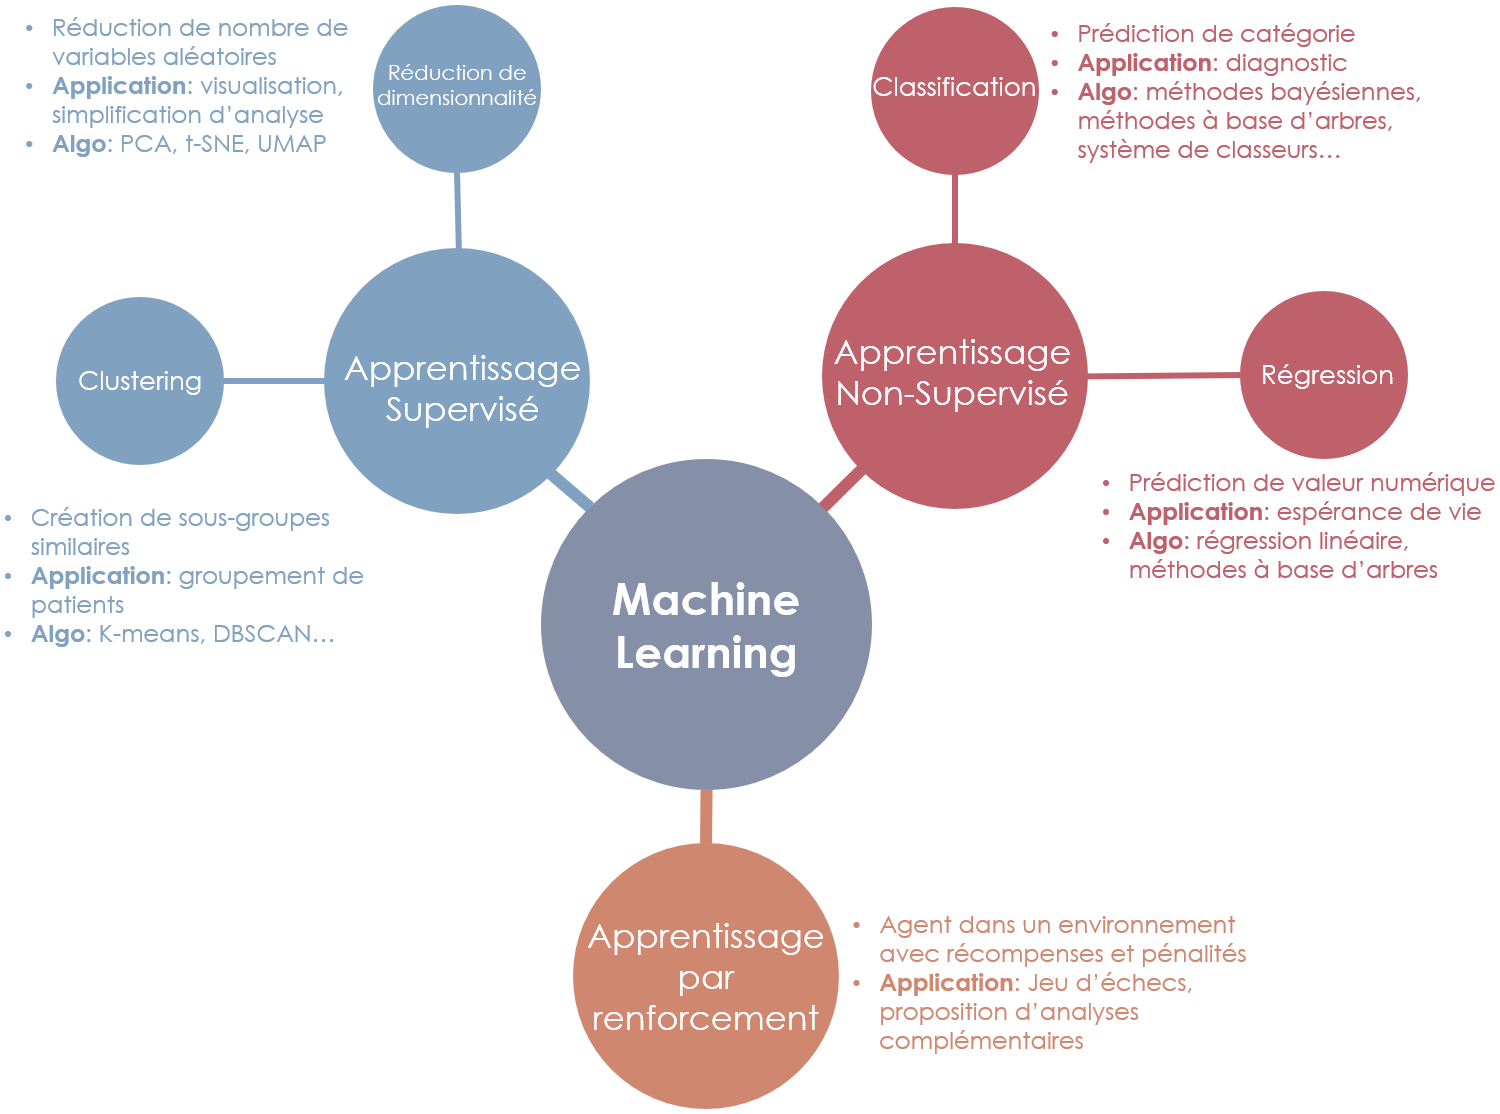
\includegraphics[width=1\textwidth]{figures/ml_landscape.png}
 \caption[Schéma des méthodes de machine-learning]{Schéma de la classification des tâches, des modes d'apprentissage et des différents cas d'applications et algorithmes associés en \textit{machine-learning}}
 \label{fig:ml-landscape}
\end{figure}

\subsection{Différents algorithmes et explicabilité}
\subsubsection{Le concept d'explicabilité}
ici on introduit quelques méthodes mais pas exhaustif
\subsubsection{Méthodes à bayesiennes}
\subsubsection{Méthodes à base d'arbres}
citer MISTIC
\subsubsection{Systèmes de classeurs}

réseaux de neuronnes après

\subsection{Limites du ML aux données biomédicales}
traitement manuel des données 
Data Integration Challenges for Machine Learning in Precision Medicine